\section{STRAT-Q, probabilistic MTP, and Test Data Governance}

\subsection{From data volume to evidence strength}

STRAT-Q treats a test result as evidence supporting or weakening a claim. Synthetic-data research therefore changes the semantics of a test campaign. The key variables are no longer only the number of cases and pass rate, but also:

\begin{itemize}[leftmargin=*]
  \item source and ancestry;
  \item degree of independence;
  \item freshness relative to the current product and deployment distribution;
  \item validity of the oracle;
  \item coverage of rare but decision-relevant regimes;
  \item contamination by the system under evaluation;
  \item synthetic generation depth;
  \item reviewer and consolidation status.
\end{itemize}

A conceptual evidence-strength function for evidence item $e$ and claim $c$ is
\[
S(e\mid c)
=Q_e F_e I_e V_e C_{e,c} T_{e,c},
\]
where $Q$ is quality, $F$ freshness, $I$ independence, $V$ verification, $C$ claim relevance, and $T$ tail coverage. This multiplicative form is illustrative; a production model should be probabilistically calibrated rather than assigned arbitrary scores.

\subsection{Evidence Passport}

A dataset, batch, or test result should carry an Evidence Passport. The passport extends dataset documentation and cryptographic provenance with decision semantics.

\begin{figure}[H]
\centering
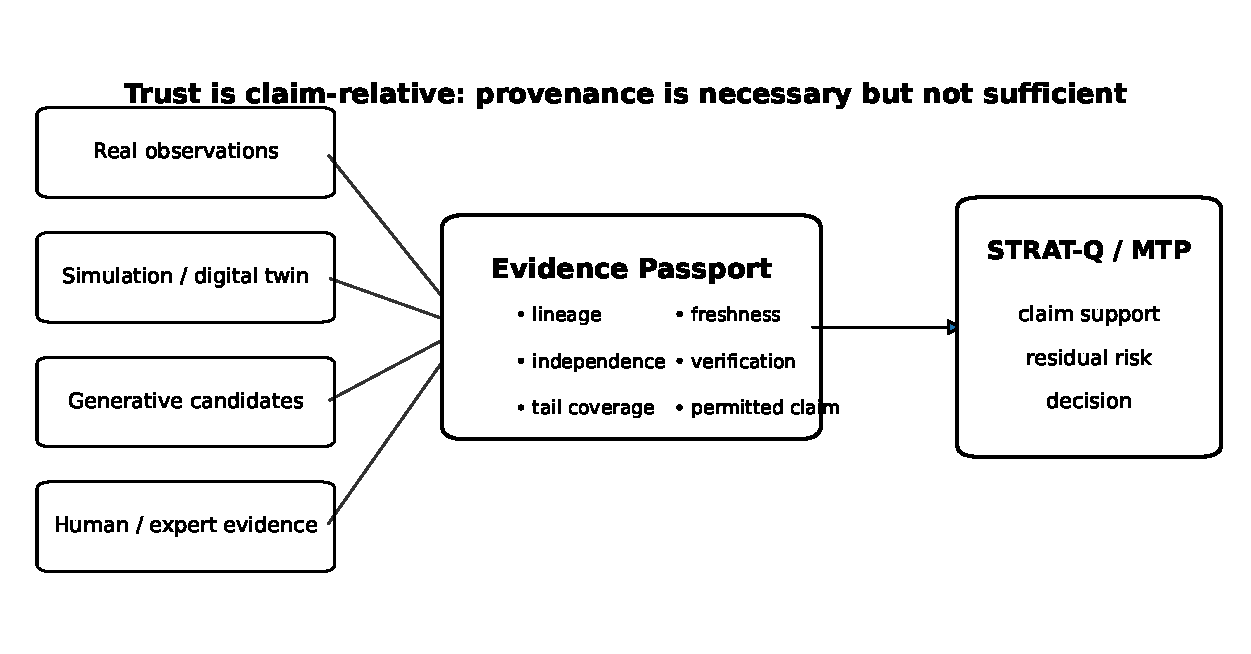
\includegraphics[width=0.95\textwidth]{figures/evidence_passport.pdf}
\caption{Evidence Passport connecting data provenance to STRAT-Q decisions.}
\label{fig:evidence-passport}
\end{figure}

Minimum fields are:

\begin{longtable}{p{0.23\textwidth}p{0.67\textwidth}}
\toprule
\textbf{Field} & \textbf{Meaning} \\
\midrule
Identity and version & Stable dataset or evidence identifier, schema version, timestamps \\
Origin class & Real observation, simulation, transformed real, generative, human review \\
Parent lineage & Parent datasets, generators, model versions, prompts, seeds, transformations \\
Generation depth & Number of generative steps since the last independent real anchor \\
Sampling policy & Temperature, top-$p$, top-$k$, rejection criteria, filtering \\
Oracle & How the expected result or validity was established \\
Verifier & Identity, independence, calibration, thresholds, false acceptance/rejection evidence \\
Freshness & Temporal, software-version, causal and distributional freshness \\
Tail coverage & Regimes covered, omitted, and intentionally oversampled \\
Permitted use & Training, exploration, regression, qualification, certification, or prohibited use \\
Supported claim & Exact claim and scope for which the evidence is relevant \\
Review status & Draft, automated-checked, expert-reviewed, approved, superseded, revoked \\
\bottomrule
\end{longtable}

\subsection{Verifiable Credentials are necessary but insufficient}

The W3C Verifiable Credentials model can establish issuer identity, integrity, status, and machine-verifiable presentation \citep{w3cvc2025}. It does not automatically establish that the content is true, current, representative, or sufficient for a decision.

We distinguish:

\begin{enumerate}[leftmargin=*]
  \item \textbf{Cryptographic verifiability:} who signed what and whether it changed;
  \item \textbf{Epistemic strength:} how reliable, independent, fresh and representative the evidence is;
  \item \textbf{Decision relevance:} whether it supports the specific claim under consideration.
\end{enumerate}

A strong signature can protect a weak dataset. Conversely, a real observation can be weak evidence if collection is biased or the deployment system has changed.

\subsection{Freshness is multidimensional}

Freshness should include:

\paragraph{Temporal freshness.} How long ago was the evidence created?

\paragraph{Version freshness.} Does it apply to the current software, model, sensor, architecture, or policy version?

\paragraph{Causal freshness.} Are the mechanisms that generated the evidence still active?

\paragraph{Distributional freshness.} Is
\[
d(P_{\mathrm{evidence}},P_{\mathrm{deploy}})
\]
within an acceptable bound?

\paragraph{Generational freshness.} How many synthetic transformations separate the evidence from an independent anchor?

A dataset generated yesterday can be generationally stale if it descends from multiple recursive teachers trained on obsolete data.

\subsection{Residual risk decomposition}

The MTP should distinguish uncertainty inside covered regimes from uncertainty due to absent regimes. A useful decomposition is
\[
R_{\mathrm{res}}
=R_{\mathrm{tested}}
+R_{\mathrm{missing}}
+R_{\mathrm{oracle}}
+R_{\mathrm{drift}}
+R_{\mathrm{dependence}}.
\]

\begin{itemize}[leftmargin=*]
  \item $R_{\mathrm{tested}}$: remaining failure risk in tested regimes;
  \item $R_{\mathrm{missing}}$: probability-weighted impact of regimes not covered;
  \item $R_{\mathrm{oracle}}$: uncertainty that expected outcomes or labels are wrong;
  \item $R_{\mathrm{drift}}$: mismatch between evidence and current deployment;
  \item $R_{\mathrm{dependence}}$: overconfidence caused by correlated evidence.
\end{itemize}

Synthetic testing often reduces $R_{\mathrm{tested}}$ efficiently. It can leave $R_{\mathrm{missing}}$ unchanged or even hidden.

\subsection{Probabilistic MTP integration}

The companion probabilistic MTP programme models incident probability as a distribution rather than a score. A simple Bayesian logistic model is
\[
\Prob(Y=1\mid X,w)
=\sigma(w^\top X+b),
\qquad
w\sim\mathcal N(\mu,\Sigma_w).
\]
The posterior is updated from test, defect, and production evidence. Synthetic-data lineage should enter either as covariates, hierarchical source effects, or likelihood weights. For source class $s$,
\[
y_j\sim\mathrm{Bernoulli}(p_j),
\qquad
\mathrm{logit}(p_j)=w^\top x_j + \alpha_{s_j},
\]
with source-specific uncertainty on $\alpha_s$.

A more explicit robust model can introduce latent label correctness $z_j$:
\[
\Prob(y_j^{\mathrm{obs}}\mid y_j^{\mathrm{true}},s_j)
\]
and infer source-specific false-label rates. This is preferable to treating a million pseudo-labels as perfect Bernoulli observations.

\subsection{Test-effort optimisation}

Let risk component $R_i^0$ be reduced by test effort $u_i$:
\[
R_i(u_i)=R_i^0e^{-\beta_i u_i}.
\]
Testing cost is
\[
C_{\mathrm{test}}(u)=\sum_i c_i u_i,
\]
and expected incident loss is
\[
C_{\mathrm{incident}}(u)
=L\sum_iR_i^0e^{-\beta_i u_i}.
\]
The optimiser solves
\[
\min_{u\ge0}
\sum_i c_i u_i
+L\sum_iR_i^0e^{-\beta_i u_i},
\]
subject to budget, calendar and resource constraints.

Synthetic data changes $\beta_i$: it may make a test category cheaper or more efficient, but only for the regimes it validly covers. We therefore replace $\beta_i$ by a posterior conditioned on evidence provenance:
\[
\beta_i\sim p(\beta_i\mid D_{\Real},D_{\Syn},V,\text{lineage}).
\]

The stopping condition remains marginal:
\[
c_i
=L R_i^0\beta_i e^{-\beta_i u_i},
\]
but uncertainty in $\beta_i$, missing-tail risk, and verification cost must be included.

\subsection{Four economic uses of test data}

A test-data budget can purchase four different things:

\begin{enumerate}[leftmargin=*]
  \item \textbf{Densification:} more confidence in an already-covered regime;
  \item \textbf{Extension:} entry into a missing or rare regime;
  \item \textbf{Refresh:} replacement of stale evidence;
  \item \textbf{Verification:} improvement of the oracle or synthetic-data reliability.
\end{enumerate}

These investments have different marginal values. The optimal test programme should choose among them rather than merely increasing execution count.

\subsection{Watermarking and provenance}

Watermarking can help detect probable synthetic origin. It does not establish truth or usefulness. A robust chain is:
\[
\text{watermark/detection}
\rightarrow
\text{provenance record}
\rightarrow
\text{credential}
\rightarrow
\text{evidence assessment}
\rightarrow
\text{decision}.
\]

The MTP should not infer ``synthetic means weak'' or ``real means strong.'' It should infer source-specific uncertainty and claim relevance.

\subsection{Reviewer and consolidation process}

Consolidation must preserve meaningful disagreement. A good evidence bundle contains:
\[
(\text{claim},\text{support},\text{contradictions},\text{scope},\text{confidence},\text{residual uncertainty}).
\]
It should not average away minority regimes. Reviewer actions should be versioned and themselves auditable.

\begin{keyidea}
Test Data Governance becomes part of the safety case. It documents not only what data exist, but why those data are allowed to reduce a specific residual risk.
\end{keyidea}
